\documentclass{beamer}
    \usetheme{Boadilla}
\usepackage{polyglossia}
    \setmainlanguage{german}
\usepackage{fontspec}
    \setsansfont{Linux Biolinum O}
\usepackage{graphicx}
\usepackage{xcolor}
\usepackage{listings}
    \lstset{language=bash,
	basicstyle=\footnotesize\ttfamily\tiny,
	breaklines=true,
	framextopmargin=50pt,
	frame=bottomline,
	backgroundcolor=\color{white!86!black},
	commentstyle=\color{blue},
	keywordstyle=\color{red},
	stringstyle=\color{orange!80!black}}
\usepackage{amsmath}
\usepackage{amssymb}
\usepackage{siunitx}
\usepackage{booktabs}
\usepackage{float}
\usepackage{tabularx}
\usepackage{caption}
\usepackage{subfig}
\usepackage{pgfplots}
    \pgfplotsset{compat=1.14}
\usepackage{hyperref}
     \hypersetup{
     colorlinks=true,
     linkcolor=black,
     filecolor=magenta}

\title{\texorpdfstring{\color{blue!50!black}\textbf{ALPIDE}}{}}
\subtitle{Threshold Scans and Noise Occupancy}
\author{Maurice Donner}
\date{21. July 2020}

\begin{document}

\maketitle

\begin{frame}{Threshold Scan}
    Inject well-defined amount of charge in a number of pixels\\
    \( \rightarrow \) Then read out hits and repeat
    \begin{itemize}
	\item Inject charge in several pixels simultaneously
	\item Use only a representative fraction of the Chip (\textasciitilde 1-5\%) \\[1cm]
    \end{itemize}
    \begin{minipage}{.35\textwidth}
	
    Parameters used:
    \begin{itemize}
	\item \texttt{PIXPERREGION 1}
	\item \texttt{NMASKSTAGES 164}
    \end{itemize}
    \end{minipage}
    \begin{minipage}{.05\textwidth}
	\ \\[0.5cm]
	\begin{tikzpicture}
	\draw[thick,black,decorate,decoration={brace}] (0,0) -- (0,-1);
    \end{tikzpicture}
    \end{minipage}
    \begin{minipage}{.57\textwidth}
    \tiny
    \ \\[0.4cm]
    Corresponds to \( 32 \cdot 164 = 5248 \) Pixels (1\% of the chip)
    \end{minipage}
\end{frame}

\begin{frame}{Threshold Scan}
    50 Injections per charge point, then plot hit probability. (S-Curve scan)\\[.5cm]
    \begin{minipage}{.49\textwidth}
	\centering
	Example:
	\begin{figure}[H]
	    \centering
	    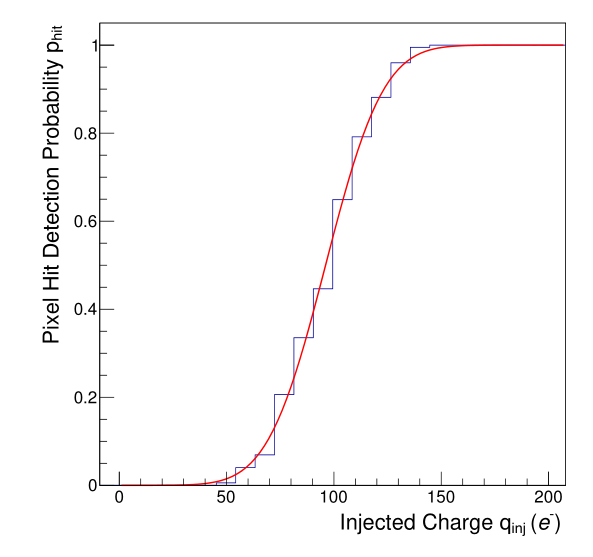
\includegraphics[width=\textwidth]{s-curve.png}
	\end{figure}
    \end{minipage}
    \begin{minipage}{.49\textwidth}
	\[ 
	   p _{\text{Hit}} (q _{\text{inj}}) = \frac{1}{2} \left(
	       1 + \text{Erf} \left[ \frac{q _{\text{inj}} - \mu}{\sqrt{2} \sigma} 
	       \right] \right)
       \]
    \end{minipage}
\end{frame}

\begin{frame}{Threshold Scan}
    \begin{minipage}{.49\textwidth}
    Distribution of Thresholds:
    \begin{figure}[H]
       \centering
       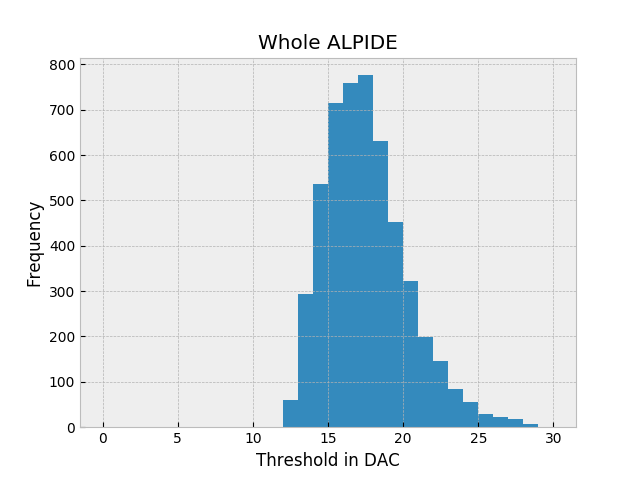
\includegraphics[trim=0 0 0 40,clip,width=.9\textwidth]{landau.png}
    \end{figure} 
    \end{minipage}
    \begin{minipage}{.49\textwidth}
	- Extract mean\\
	\pause
	- Repeat with different settings and compare the runs
	\begin{figure}[H]
	    \centering
	    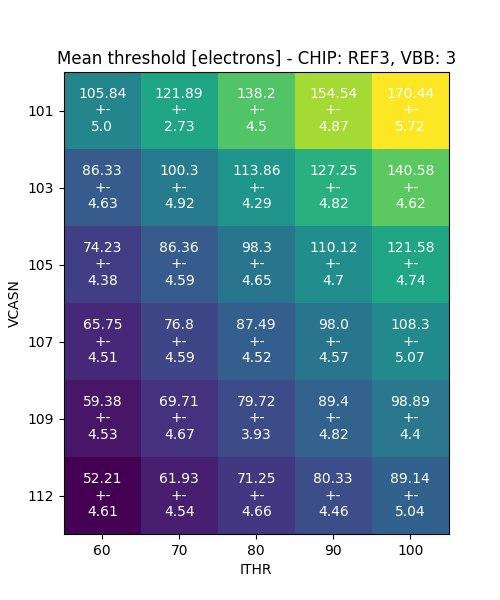
\includegraphics[trim=0 0 0 50, clip, width=.9\textwidth]{thresholdmap.jpg}
	\end{figure}
	\tiny VCASN and ITHR are the main parameters to modify the Threshold
    \end{minipage}
    \pause
    For cosmic muons at 50 GeV:
    Energy Deposit \textasciitilde 0.0286 MeV\\
    7900 e-h-pairs
\end{frame}

\begin{frame}{Noiseoccupancy Scan}
    Gives a selectable number of triggers and returns the number of hits.
    \begin{itemize}
	\item If Threshold is low enough for electronic noise to produce a hit,
	    measurements taken will be affected by a fake hit rate.
    \end{itemize}
    \pause
    \begin{figure}[H]
	\centering
	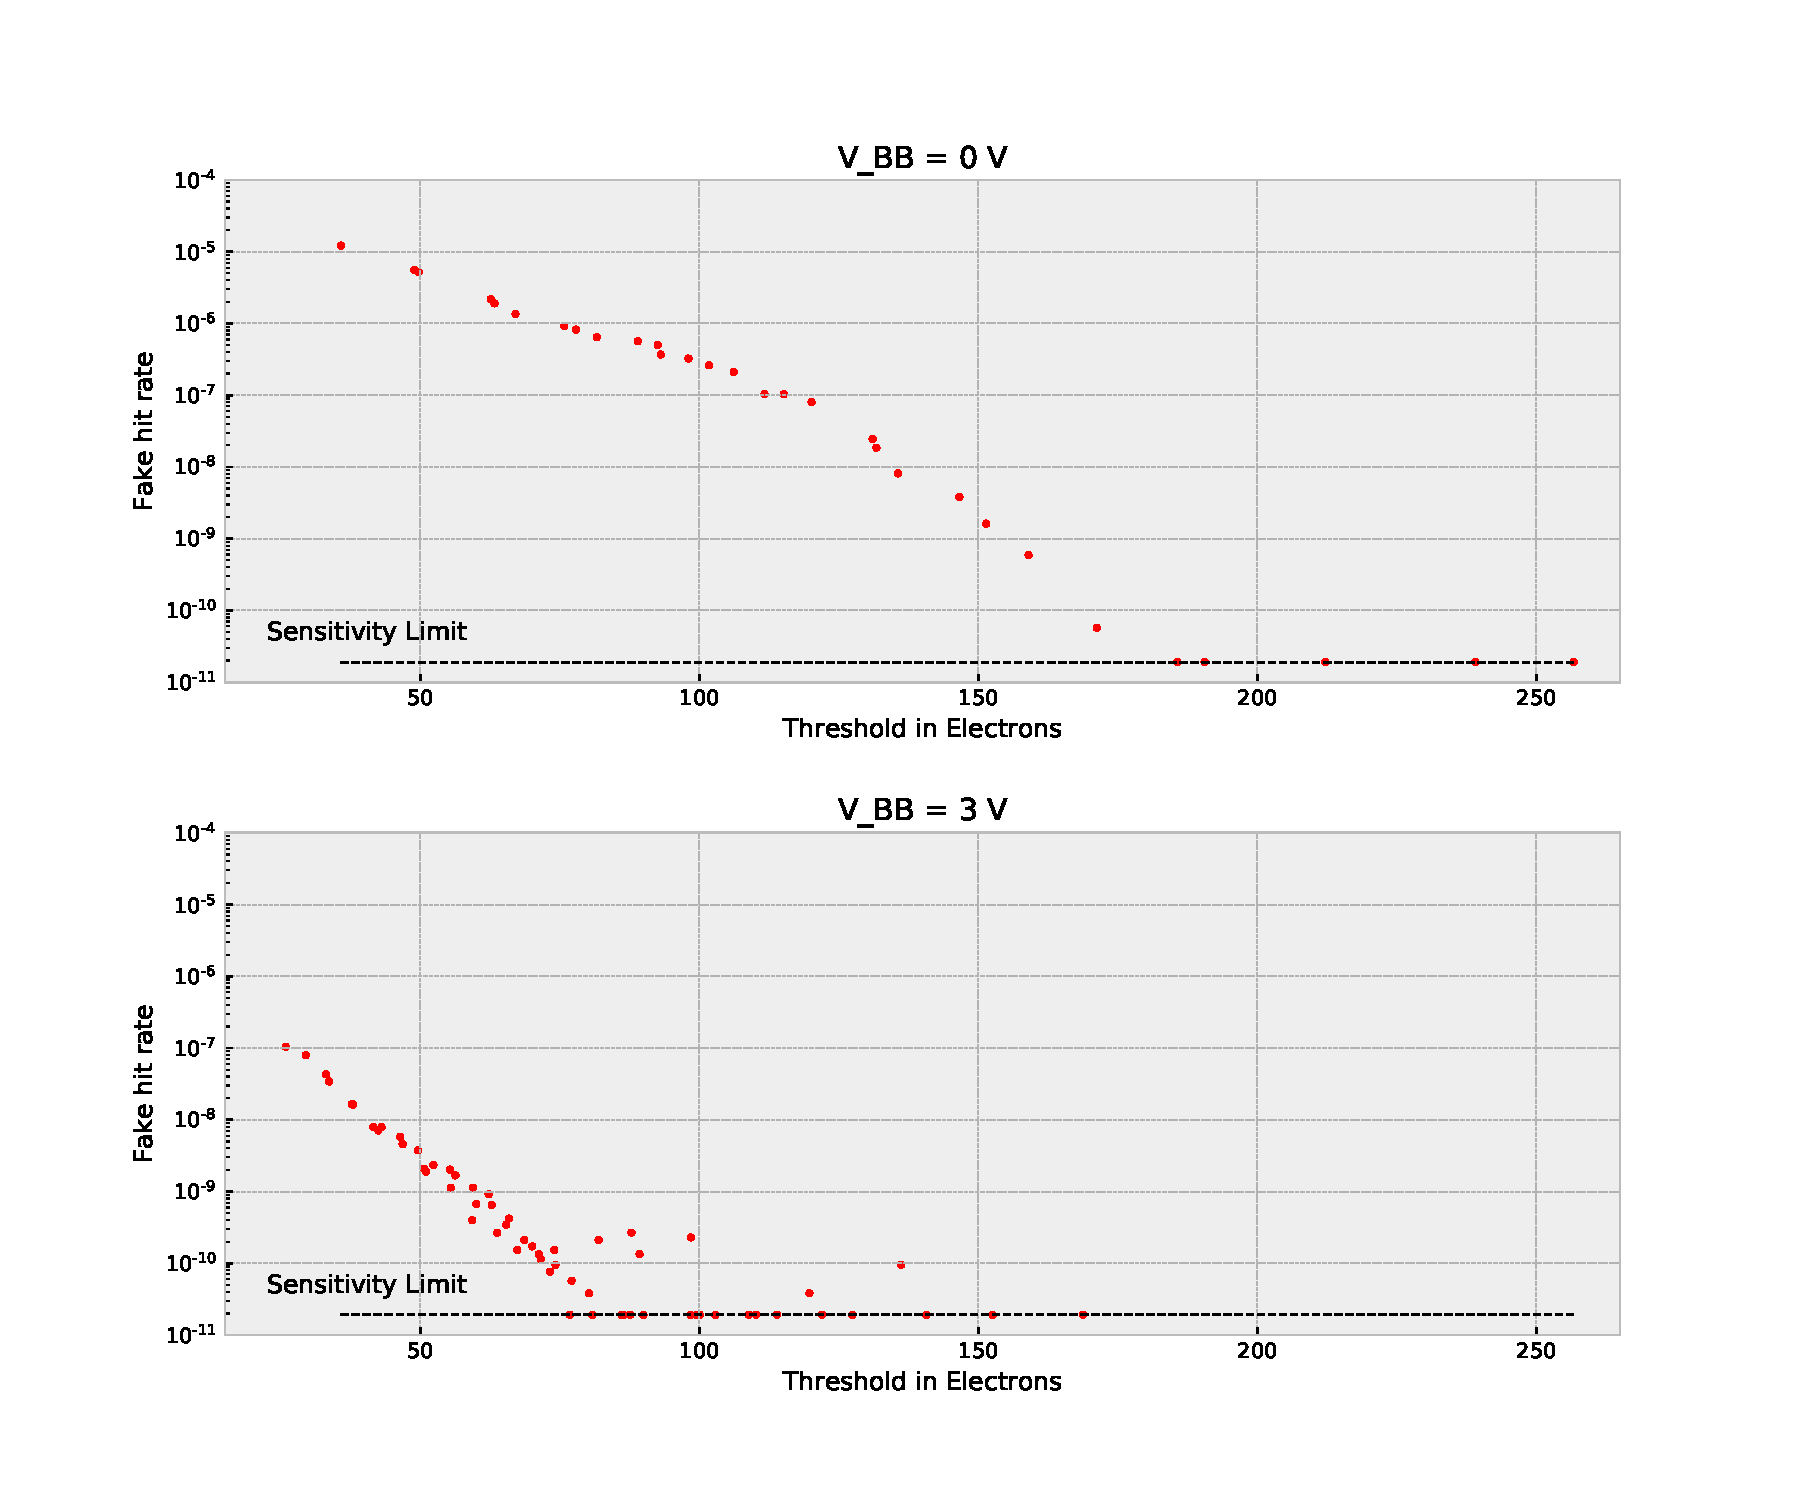
\includegraphics[trim=0 360 0 70, clip, width=\textwidth]{Fake_Hit_Rate.pdf}
    \end{figure}
\end{frame}

\begin{frame}{Noiseoccupancy Scan}
    Gives a selectable number of random triggers and returns the number of hits.
    \begin{itemize}
	\item If Threshold is low enough for electronic noise to produce a hit,
	    measurements taken will be affected by a fake hit rate.
    \end{itemize}
    \begin{figure}[H]
	\centering
	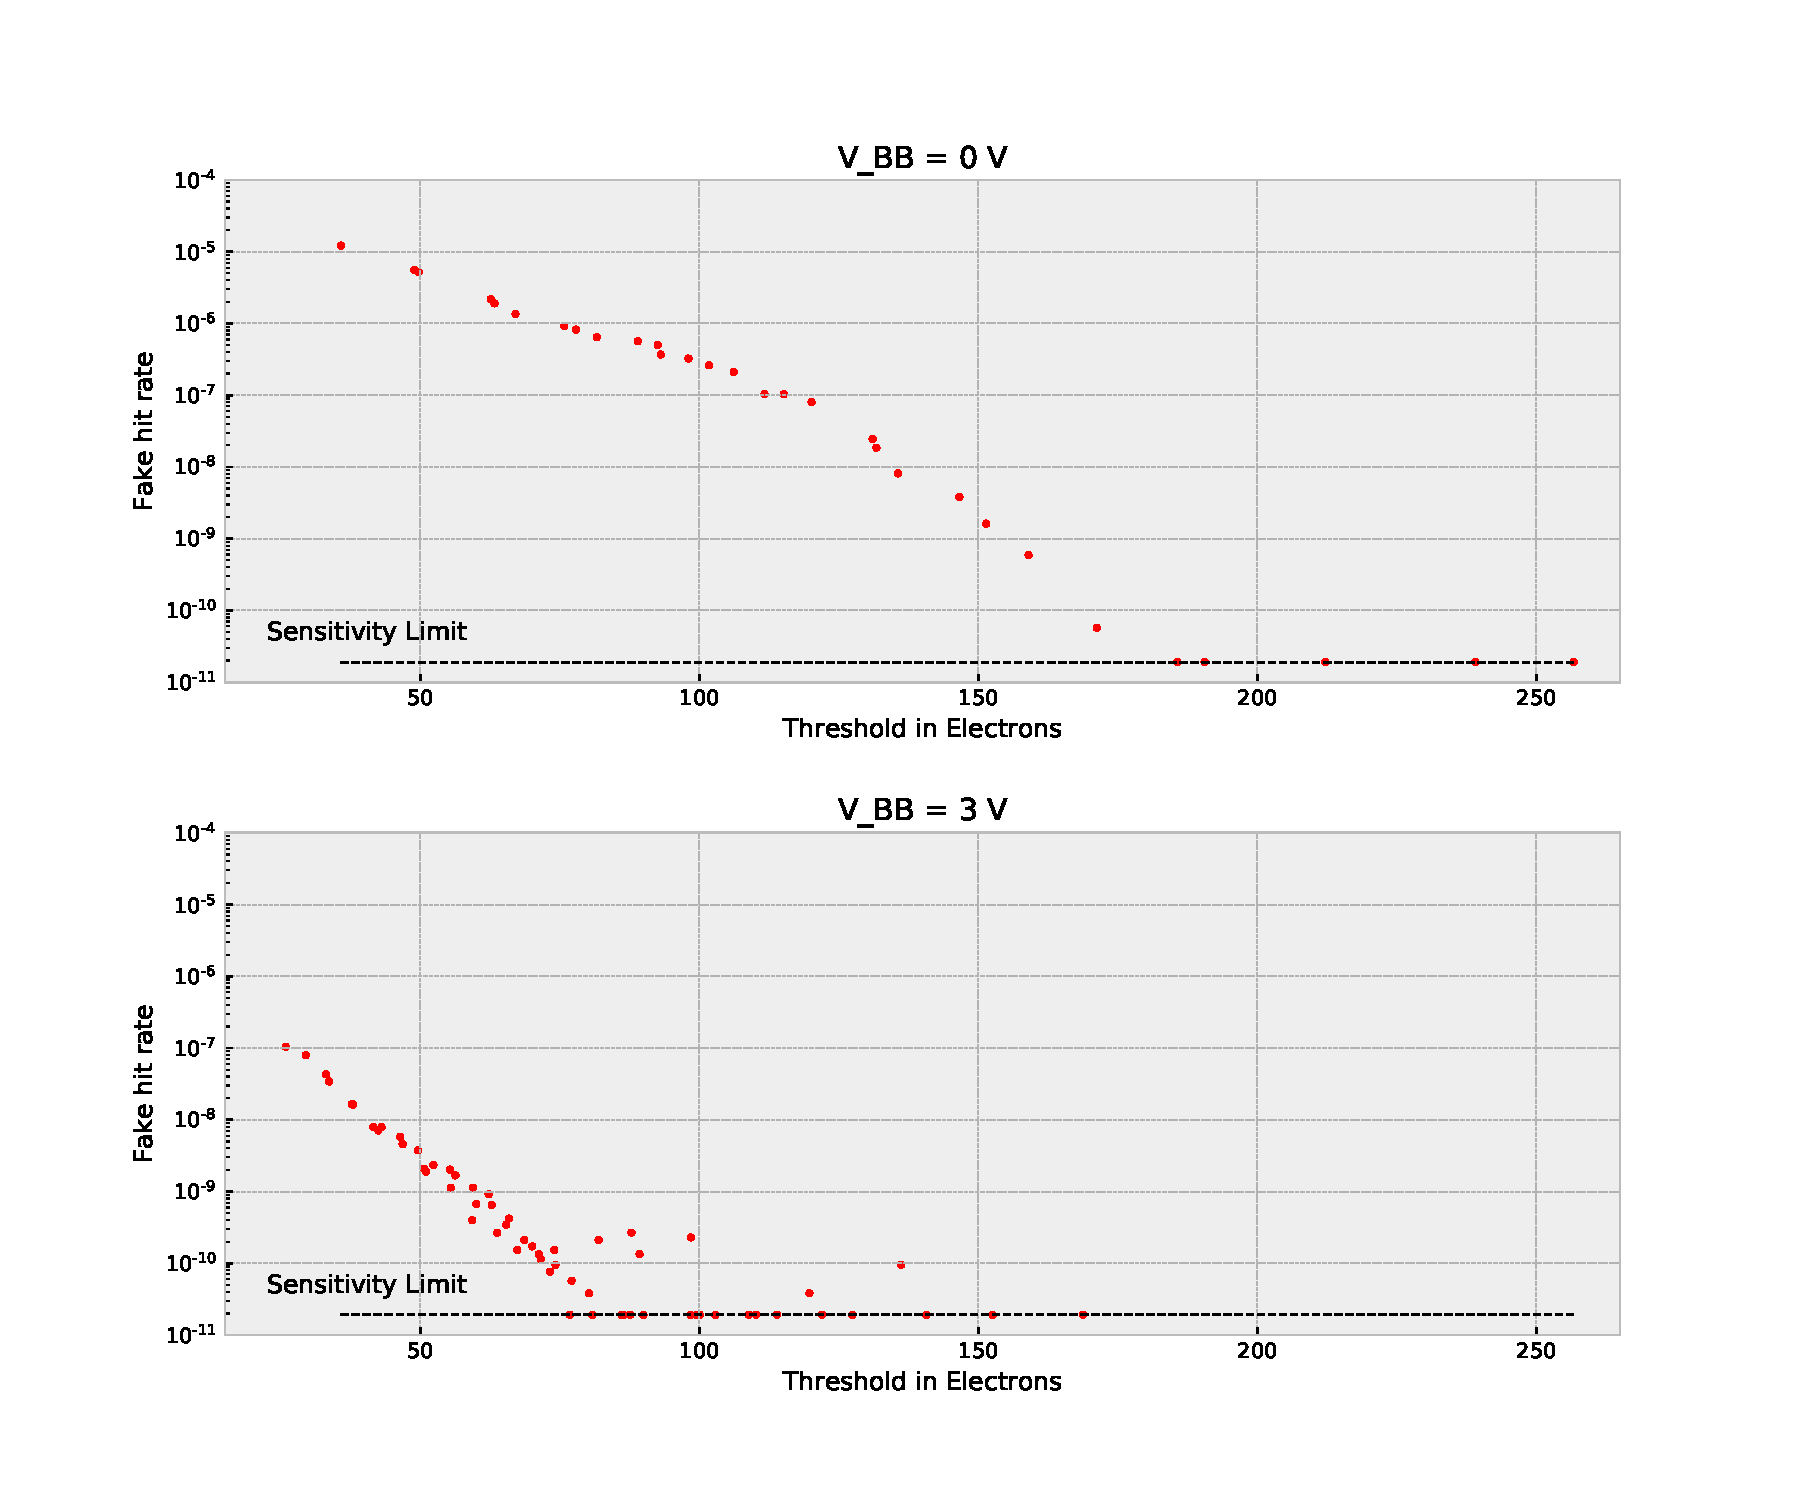
\includegraphics[trim=0 50 0 380, clip, width=\textwidth]{Fake_Hit_Rate.pdf}
    \end{figure}
\end{frame}

%\begin{frame}{}
%    Hit probability (Fake Hit rate): Integrate 
%    \[
%	p ^{\text{expected}} _{\text{FH}} =
%	\frac{1}{2} \text{Erfc} \left[ \frac{\mu}{\sqrt{2} \cdot \sigma} \right]
%    \]
%    from the threshold \( \mu \) to \( \infty \) 
%\end{frame}

\end{document}
